Here we detail our most complex experiment. This time we aimed to (almost) cancel any kind of dependence from parameters. The idea is that we will let a regression chose whether to switch a strategy on or off. The potential advantages of such methods are multiple: in fact reducing the dependence from parameters we basically cancel the possibility of overfitting, while letting a model work on the processed information allows to extract more information out of the PnL curve. We will not try any complex Machine Learning method as we don't want something very obscure and hard to interpret, but moreover we need something extremely fast. The idea is that every Monday we will fit a linear model to the data available up to that day, then we will make a prediction looking at the data we have at that current moment in time. If the prediction is good we will put the strategy in production, otherwise we will leave it switched off.\\
The linear model that we will fit is the following:

\begin{equation} \label{OLS}
r_i = \alpha + \beta_1 Sharpe_{long,i} + \beta_2 Sharpe_{mid,i} + \beta_3 Sharpe_{short,i}  + \epsilon_i 
\end{equation}

Where $r_i$ stands for the daily return of a trading strategy and the various Sharpe ratios stand for a rolling sharpe computed on the data up to that day. With this model we aim to capture information from long and short term together. Of course there are some details to be fixed before proceeding. For example the OLS framework assumes that our data is normally distributed, unfortunately as we noticed in section 2 our data is not Gaussian. Each day we will standardize our data with mean and variance available up to that day, in this way our regression will be more meaningful.\\
There is an additional layer of filtering that we want to use, and it is relative to the fact that not all strategies can be suitably switchable with this model, what we will do then is to require for each regression that we run to have at least one of the $\beta s$ of the regressions to be statistically significant at a 95\% level(i.e. with a t-stat of at least 1.65).\\
This model is definitely more robust, the only parameter we have is the threshold on the prediction of the regression used to define a strategy as "good", but it will be calibrated in a way that we reach a certain number of strategies in production. The other parameters are the windows of the Sharpe ratios, but these are quite simple to choose once we have seen the results of the Random Forest, it makes sense to take as windows for the three Sharpe ratios 350, 180 and 60 respectively.\\
One last  consideration to be made is relative to a weak point of this method, since we are regressing many strategies, our model will take a long time to be backtested. For each backtest (in-sample) we roughly have to run $13000 \cdot 395 = 5135000$ regressions.\\
But let's move to explore the results of this model. 

\begin{table}
	\centering
	\begin{tabular}{c|c}
		\textbf{Statistic} & \textbf{Value} \\\hline
		Sharpe Ratio & 2.235 \\ 
		Sortino Ratio & 2.5471 \\ 
		Omega Ratio & 1.53 \\ 
		Skewness & -0.7782 \\ 
		Kurtosis & 11.20 \\ 
		Maximum Drawdown (\% duration/duration) & 10.6 \\ 
		Longest Drawdown (days) & 88.0 \\ 
		Winning Days & 61.47 \\ 
	\end{tabular}
	\caption{\label{tab:widgets} Statistics for the in-sample performance of the Regression based method.}
\end{table}

We can see that unfortunately the robustness given by this model is not matched by a good performance as well. Even though the method might be good we decided to drop it due to the bad performance it provides.  

\begin{center}
	\centering
	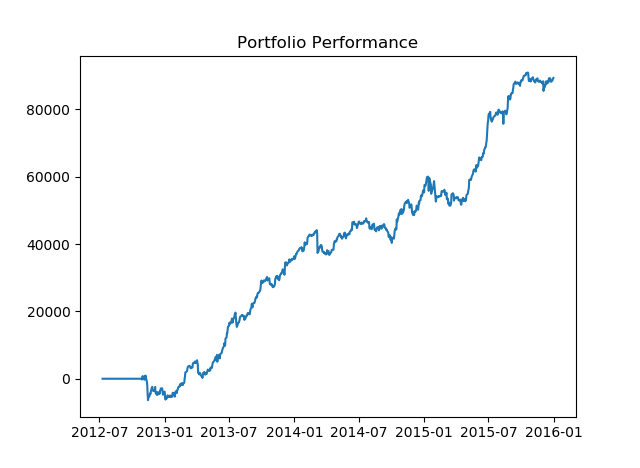
\includegraphics[width=0.6\textwidth]{GridSearches/Regression_Based/in_sample_performance.png}
	\captionof{figure}{In-sample performance of the Regression based method}
	\label{Average_Drawdown_3}
\end{center}


\begin{center}
	\centering
	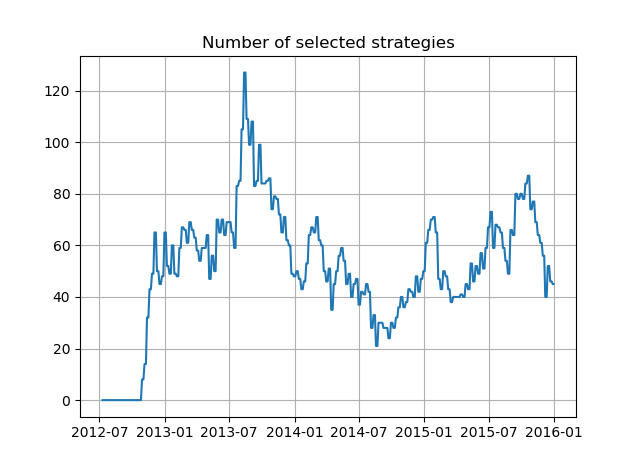
\includegraphics[width=0.6\textwidth]{GridSearches/Regression_Based/num_strats_in_sample.png}
	\captionof{figure}{Number of strategies selected each week by the Regression based method.}
	\label{Average_Drawdown_in_sample}
\end{center}

As we can see, here we select more strategies than before, but the performance is still subject to many drops that really make us not favour this model over the other ones.